\chapter{Chapter B}\label{app:BB}
\section{PhP URLs code}
\begin{lstlisting}[style=php, caption={PHP URLs code}]
<?php

// Create Post
URL:/posts/create
Method:{POST}
Description: Allows a student to create a new post.
Request Body: JSON containing post details.
Authorization: Requires a valid authentication token.

// Apply for Post
URL:/posts/\{post\}/apply
Method:{POST}
Description: Allows a student to apply for a specific post.
URL Parameters: ID of the post.
Authorization: Requires a valid authentication token.

// Update Post
URL:/posts/\{id\}/update
Method:{PUT}
Description: Allows updating an existing post.
URL Parameters: ID of the post.
Request Body: JSON containing updated post details.
Authorization: Requires a valid authentication token.

// Delete Post
URL:/posts/\{post\}/delete
Method:{DELETE}
Description: Allows deleting an existing post.
URL Parameters: ID of the post.
Authorization: Requires a valid authentication token.

// Search Questions
URL:/questions/search
Method:{GET}
Description: Allows searching for questions based on criteria.
Query Parameters: Keywords for search.
Authorization: Requires a valid authentication token.

// Retrieve All Questions
URL:questions/all
Method:{GET}
Description: Retrieves all questions in the system.
Authorization: Requires a valid authentication token.

// Create Question
URL:/questions/create
Method:{POST}
Description: Allows a student to create a new question.
Request Body: JSON containing question details.
Authorization: Requires a valid authentication token.

// Rate Question
URL:/questions/\{id\}/rate
Method:{POST}
Description: Allows a student to rate a specific question.
URL Parameters: ID of the question.
Request Body: JSON containing rating details (+1 for like, -1 for dislike).
Authorization: Requires a valid authentication token.

// Update Question
URL:/questions/\{id\}/update
Method:{PUT}
Description: Allows updating an existing question.
URL Parameters: ID of the question.
Request Body: JSON containing updated question details.
Authorization: Requires a valid authentication token.

// Delete Question
URL:/questions/\{id\}/delete
Method:{DELETE}
Description: Allows deleting an existing question.
URL Parameters: ID of the question.
Authorization: Requires a valid authentication token.

// Retrieve Profile
URL:/student/profile
Method:{GET}
Description: Retrieves the profile of the authenticated student.
Authorization: Requires a valid authentication token.

// Update Profile
URL:/student/profile/update
Method:{PUT}
Description: Allows updating the profile of the authenticated student.
Request Body JSON containing updated profile details.
Authorization: Requires a valid authentication token.
\end{lstlisting}

\section{Pagination in Back - end}
\begin{figure}[H]\label{fig:pagination}
  \centering
  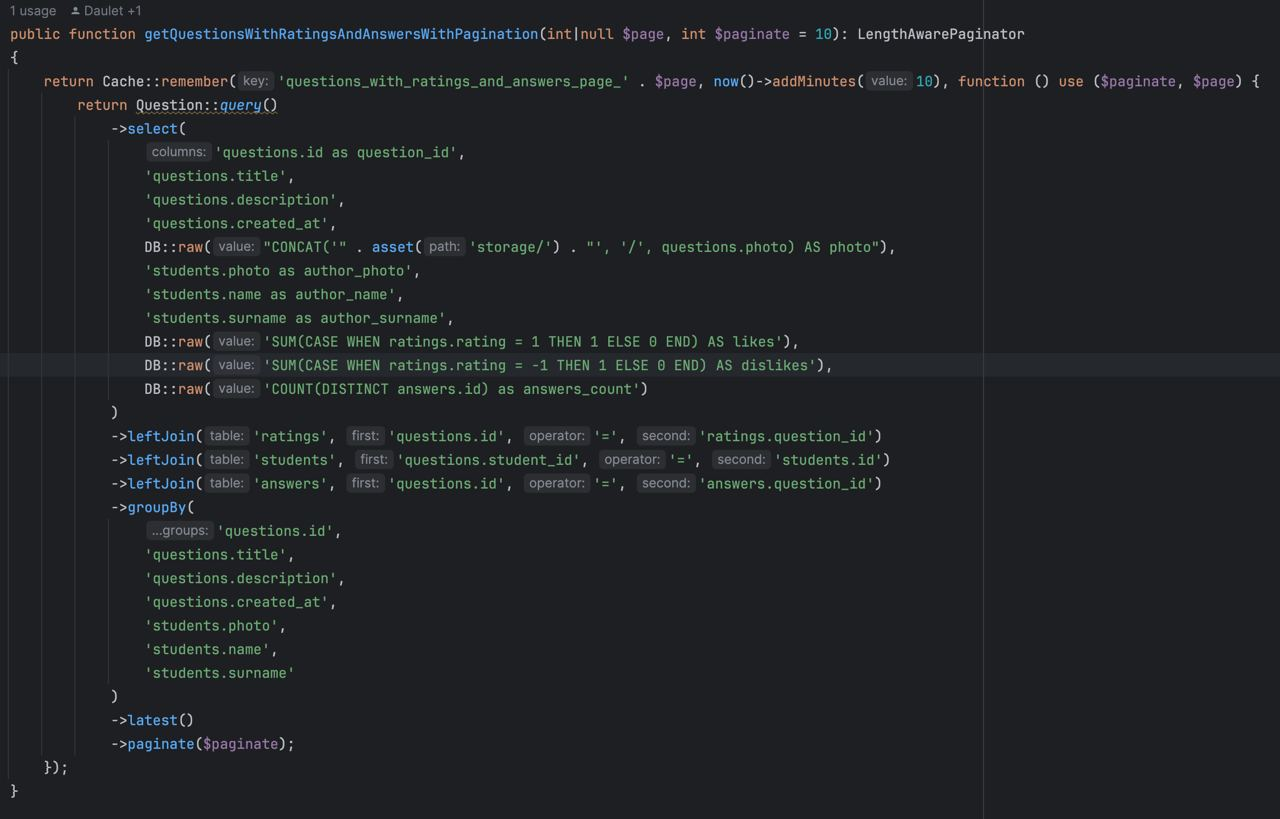
\includegraphics[width=0.8\linewidth]{figures/Pagination.jpg}
  \caption{Pagination.}
\end{figure}
\section{IOS Screens of codes}
\begin{figure}[H]\label{fig:authorization}
  \centering
  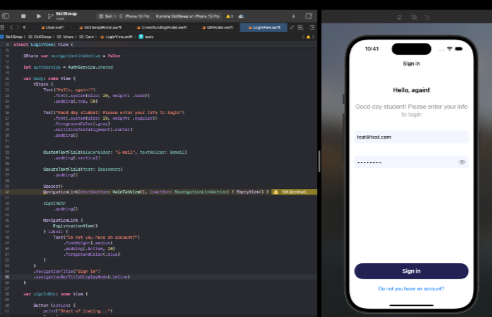
\includegraphics[width=0.8\linewidth]{figures/Authorization.png}
  \caption{Authorization.}
\end{figure}
\begin{figure}[H]\label{fig:skillsharingmodel}
  \centering
  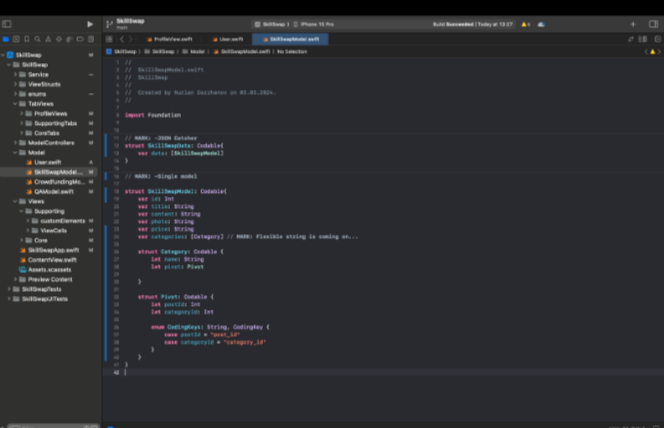
\includegraphics[width=0.8\linewidth]{figures/Skill Sharing model.png}
  \caption{Skill Sharing model.}
\end{figure}
\begin{figure}[H]\label{fig:crowdfundingmodel}
  \centering
  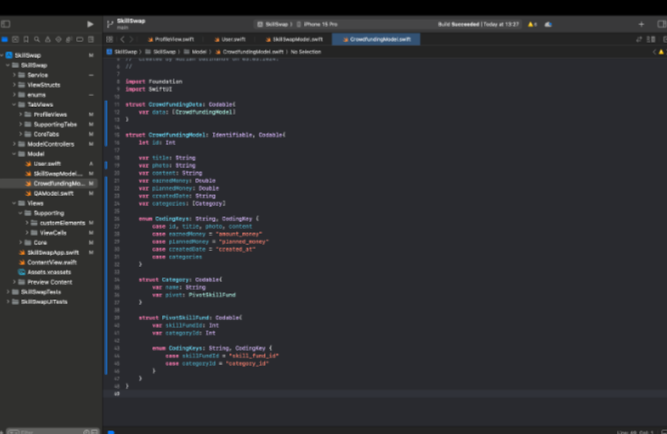
\includegraphics[width=0.8\linewidth]{figures/Crowdfunding model.png}
  \caption{Crowdfunding model.}
\end{figure}
\begin{figure}[H]\label{fig:questionanswerModel}
  \centering
  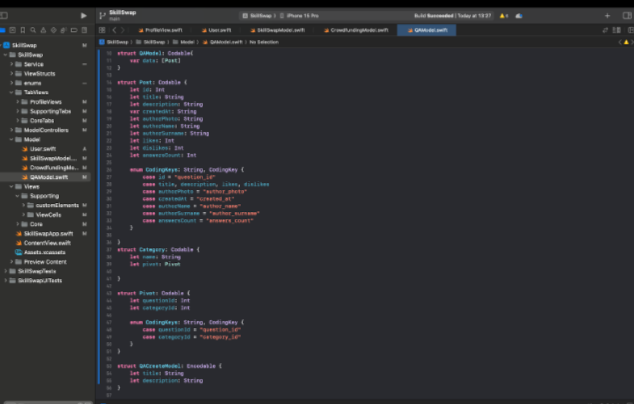
\includegraphics[width=0.8\linewidth]{figures/Question and Answer (QA) Model.png}
  \caption{Question and Answer (QA) Model.}
\end{figure}
\begin{figure}[H]\label{fig:registration}
  \centering
  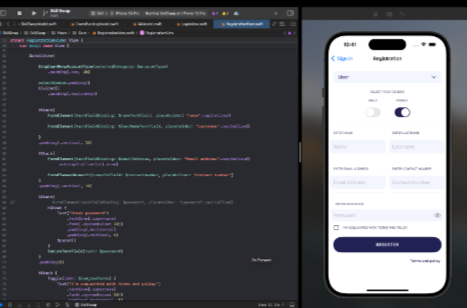
\includegraphics[width=0.8\linewidth]{figures/Registration.png}
  \caption{Registration.}
\end{figure}
\begin{figure}[H]\label{fig:authorizationmodel}
  \centering
  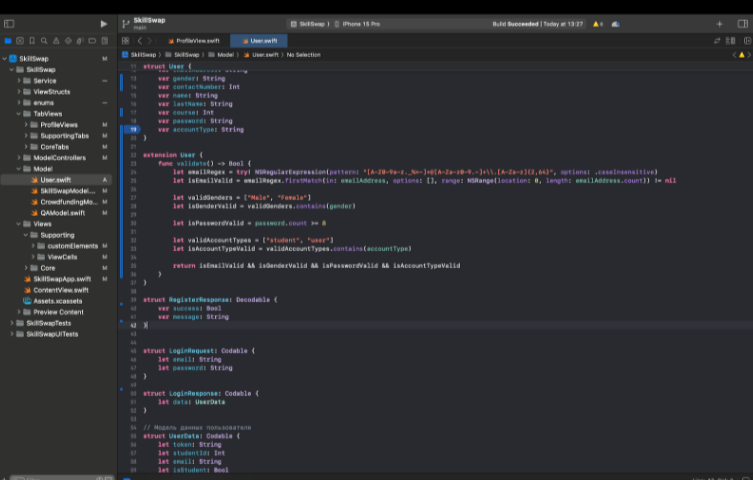
\includegraphics[width=0.8\linewidth]{figures/Authorization model.png}
  \caption{Authorization model.}
\end{figure}
\begin{figure}[H]\label{fig:createpstskillswap}
  \centering
  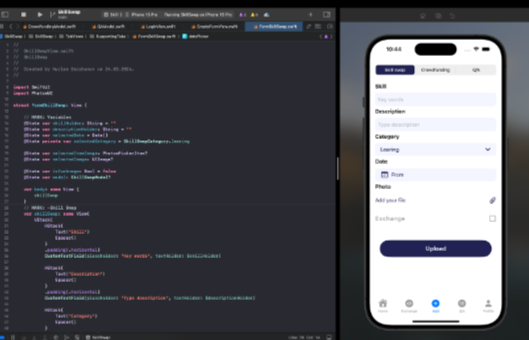
\includegraphics[width=0.8\linewidth]{figures/Creating a post (Skill Swap).png}
  \caption{Creating a post (Skill Swap).}
\end{figure}
\begin{figure}[H]\label{fig:createpstcrowd}
  \centering
  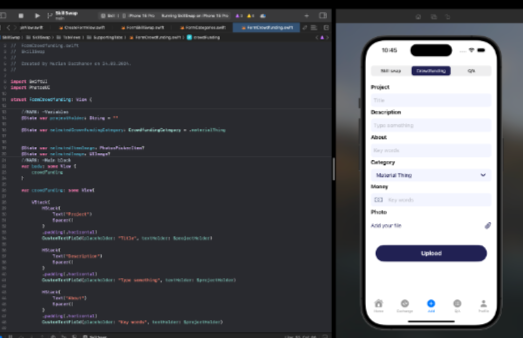
\includegraphics[width=0.8\linewidth]{figures/Create a post (Crowdfund).png}
  \caption{Create a post (Crowdfund).}
\end{figure}
\begin{figure}[H]\label{fig:createpstq}
  \centering
  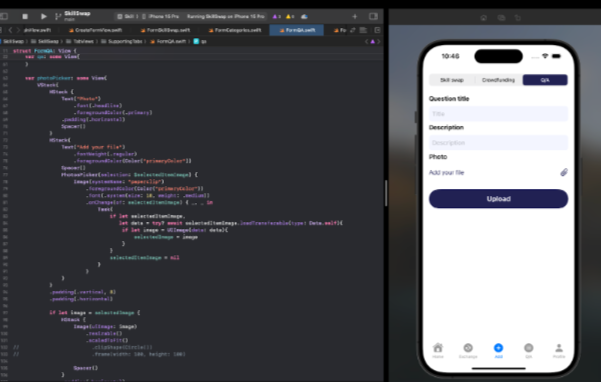
\includegraphics[width=0.8\linewidth]{figures/Crate a post (Question).png}
  \caption{Crate a post (Question).}
\end{figure}